% fig-cep-conditions — §5.1, the five CEP conditions combined (AND).
% Standalone-buildable AND \input-able. Uniform condition boxes, muted palette,
% the AND-gate (the conjunction = the load-bearing element) accented.
\documentclass[border=4pt]{standalone}
\usepackage{tikz}
\usetikzlibrary{positioning,arrows.meta}
% figures/colors.tex — shared, muted, arXiv-safe palette for all four figures.
% Change colours HERE; all four figures + the paper pick it up.
% Requires xcolor (loaded by tikz / the paper). \input-able in a preamble.
\definecolor{figline}{HTML}{3A4A5A}        % muted slate-blue — outlines + text (standard)
\definecolor{figfill}{HTML}{ECF1F6}        % very light blue-grey — standard node fill
\definecolor{figaccent}{HTML}{2E6E66}      % muted teal — central / key element outline
\definecolor{figaccentfill}{HTML}{DBEAE6}  % light teal — central element fill
\definecolor{figmuted}{HTML}{6B7785}       % muted grey — labels / secondary text

\begin{document}
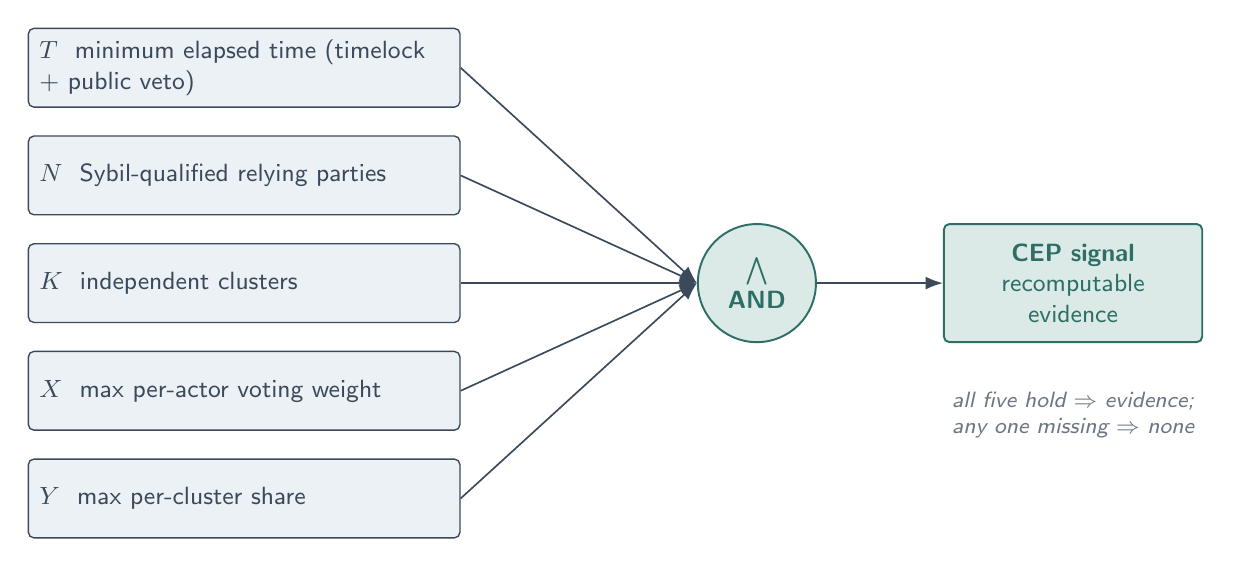
\begin{tikzpicture}[
  cond/.style={draw=figline, line width=0.5pt, rounded corners=2pt, align=left,
               text=figline, font=\small\sffamily, fill=figfill,
               text width=52mm, minimum height=10mm, inner sep=4pt},
  gate/.style={draw=figaccent, line width=0.7pt, circle, text=figaccent,
               font=\small\sffamily\bfseries, minimum size=15mm, fill=figaccentfill, align=center},
  obox/.style={draw=figaccent, line width=0.7pt, rounded corners=2pt, align=center,
               text=figaccent, font=\small\sffamily, fill=figaccentfill,
               text width=30mm, minimum height=15mm, inner sep=4pt},
  flow/.style={-{Latex[length=2.2mm]}, draw=figline, line width=0.6pt},
  node distance=3.5mm
]
\node[cond] (c1) {$T$\ \ minimum elapsed time (timelock + public veto)};
\node[cond, below=of c1] (c2) {$N$\ \ Sybil-qualified relying parties};
\node[cond, below=of c2] (c3) {$K$\ \ independent clusters};
\node[cond, below=of c3] (c4) {$X$\ \ max per-actor voting weight};
\node[cond, below=of c4] (c5) {$Y$\ \ max per-cluster share};
\node[gate, right=30mm of c3] (and) {$\bigwedge$\\AND};
\node[obox, right=16mm of and] (sig) {\textbf{CEP signal}\\recomputable evidence};
\foreach \c in {c1,c2,c3,c4,c5} \draw[flow] (\c.east) -- (and.west);
\draw[flow] (and) -- (sig);
\node[font=\footnotesize\sffamily\itshape, text=figmuted, below=5mm of sig,
      text width=36mm, align=center]
     {all five hold $\Rightarrow$ evidence;\\ any one missing $\Rightarrow$ none};
\end{tikzpicture}
\end{document}
